%-------------------------------%
\begin{figure}[ht]
\centering
    %\newcommand{\scaleFactor}{1.3} % Define the scale factor
    \newcommand{\gridgreenredblack}{\foreach \x in {0,1,2,3}{\foreach \y in {0,1,2}	\node[box] at (\x,\y){};}
        \node[box, fill=green] at (3,2){{\boldmath $+1$}};
        \node[box, fill=red] at (3,1){{\boldmath $-1$}};
        \node[box, fill=black] at (1,1){};
    }
    \scalebox{1.5}{
            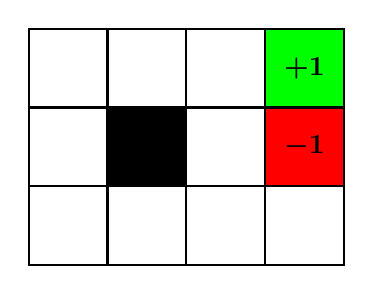
\begin{tikzpicture}
                [box/.style={rectangle,draw=black,thick, minimum size=1cm},
                arrow/.style={->,>=stealth,very thick},
                ]
                \gridgreenredblack
            \end{tikzpicture}
    }
    \caption{The slippery gridworld environment. The agent can move in any of the four cardinal directions. Receives reward (punishment?) $\epsilon<0$ on each timestep. Movement is noisy, with a 70\% chance of moving in the desired direction, and 10\% of moving in the other three directions. Episode ends when the agent lands in \textbf{heaven} 
            \tikz[baseline=-0.5ex] \node[rectangle, draw=black, fill=green, inner sep=2pt] {\textbf{+1}};
            (and gets reward +1) or in \textbf{hell}
            \tikz[baseline=-0.5ex] \node[rectangle, draw=black, fill=red, inner sep=2pt] {\textbf{-1}};
			(and gets reward -1).
            The wall \tikz[baseline=-0.5ex] \node[rectangle, draw=black, fill=black, inner sep=2pt] {\textbf{-1}}; is impassible;
            any movement that would walk into the wall, or off the grid, has no effect.}
    \label{fig:gridworld}
\end{figure}